\part{Introduction} % (fold)
\label{prt:introduction}
\chapter{Preface} % (fold)
\label{cha:preface}
This thesis discusses early measurements taken at the MuSIC beam-line. MuSIC is a new muon source at the Research Centre for Nuclear Physics (RCNP) in Osaka, Japan. Commissioning of the beam began in 2010 with installation of the Pion Capture Solenoid (PCS) and the first 36\(^{\circ}\) of Muon Transport Solenoid (MTS).

While still incomplete, enough of MuSIC exists to test the efficacy of the PCS. The PCS uses a novel design in order to to maximise muon production which is predicted to be several orders of magnitude more effective than the generation of capture solenoids. This thesis is concerned with the early measurements made at MuSIC towards characterising the beam and testing the validity of this new design.

In exploring this premise this thesis is divided into three core parts: this part (the introduction, part~\ref{prt:introduction}), discussion of the simulation (part~\ref{prt:simulation}) and discussion of the measurements made to characterise the beam (part~\ref{prt:characterising_the_beam}). There is an additional part (part~\ref{prt:lpd_ccc_interface}) which is an appendix discussing some parallel work that was carried out in designing the firmware interface between the `Clock and Control Card' (CCC) and the `Large Pixel Detector' (LPD) for the `European X-ray Free Electron Laser' (EuXFEL).

The rest of this part begins with a discussion of the motivation for high intensity (and hence high efficiency) muon sources, then discussion of the specific motivation for MuSIC and finally a brief review of the physical processes required to understand the rest of this thesis.

% chapter preface (end)
%%%%%%%%%%%%%%%%%%%%%%%%%%%%%%%%%%%%%%%%%%%%%%%%%%%
\chapter{High Intensity Muon Sources} % (fold)
\label{cha:high_intensity_muon_sources}
As well as being an interesting particle in its own right, muons have several properties that make them useful as a tool for further research. Muons are 500 times more massive than their sibling, the electron, so they lose less energy through synchrotron radiation making them excellent probes. The primary problem with using muons as a probe is that, unlike electrons, they decay; with a lifetime of 2.1969811\( \pm \)0.0000022~\( \mu \)s~\cite{PDG for muons} they are much more difficult to manipulate than the, comparatively immortal, electron. Due to the difficulty of manipulating and accelerating a muon beam before it decays, electrons have been the `go to' lepton but with accelerator systems growing ever larger (the International Linear Collider is predicted to be 31~Km long~\cite{International Linear Collider ref}) there has been growing interest in moving to, smaller, muon technologies. 

As short lived particles muons cannot be produced in the same was as, for example, electrons: through ionisation and then acceleration. The most common method for production is pion decay (see figure~\ref{fig:pion_decay_feyman}), this process produces muons 99.98770$\pm$0.00004~\%~\cite{PDG CITATION PLEASE} of the time.\footnote{The next most common decays are \( \pi\rightarrow\mu\nu_{\mu}\gamma \) and \( \pi\rightarrow e \nu_e \); \( (2.00\pm0.25)\times10^{-4} \)\% and \( (1.230\pm0.004)\times10^{-4} \)\% of time respectively.} The pion has a lifetime of only 26.033\(\pm\)0.005~ns~\cite{PDG for pions}, i.e.\ \( \sim \)1\% of the lifetime of the muon meaning that, given a suitably long decay pipe, the pion contamination of the muon beam can be kept low. The production of pions is a more complex hadronic process, that is beyond the scope of this thesis, but can be summarised as the result of proton-proton interactions above the threshold energy of 380~MeV. The simplest method of creating proton-proton interactions is through use of a fixed target that a proton beam is incident upon.

\begin{figure}[hptb]
  \centering  
    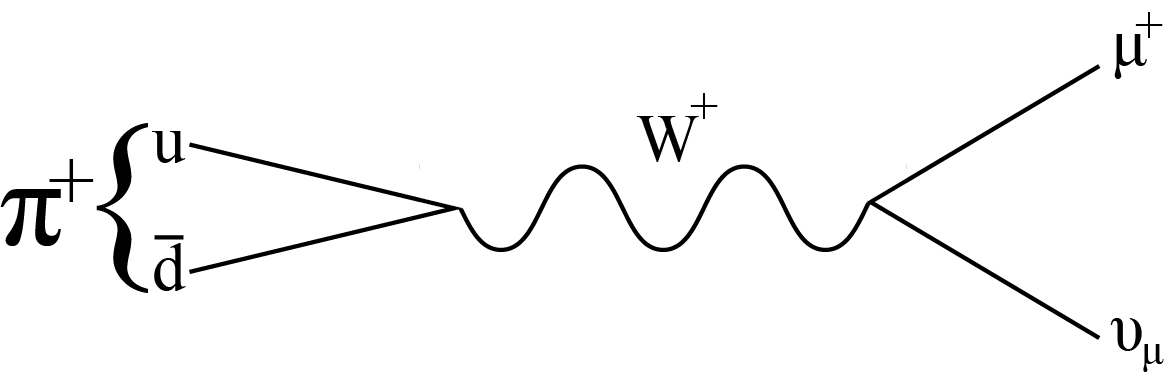
\includegraphics[scale=0.8]{images/pion_decay_feyman.png}
  \caption{Feynman diagram showing muon production through pion decay.}
  \label{fig:pion_decay_feyman}
\end{figure}

Whilst all muon sources use pion decays to generate their beams there are several broad categories of beam. Muon beams are generally categorised depending on where the muons originate: `decay', `cloud', `surface' and `sub-surface'. Most muon facilities will have one or more of each type of beam, as they are not incompatible and all have different properties. The simplest category of beam is made from `decay' muons, in this case pions care captured and transported to a decay pipe to produce both forward and backward travelling muons. `Cloud' muon beams collect muons produced by pion decay close to the proton-stopping target, in general they have a higher flux than decay type beams due to the increased collection efficiency. `Surface' and `sub-surface' beams are both generally of lower momenta (\( <30\)~MeV/c) than cloud and decay types as they collect positive muons produced by pions decaying at rest on the surface (or just inside of it) of the target, these beams are in high demand by muon spin resonance (\(\mu\)SR) experiments as they require high fluxes of stopping (i.e.\ low momenta) muons.

There are currently several dedicated muon sources\footnote{In theory any proton source, with energy above the pion production threshold, can operate as a muon source but only a few have dedicated facilities.} around the world (see table~\ref{tab:cf_muon_sources}). All of the current muon sources have their facilities acting in a parasitic mode on their main proton beam-line, with the majority of the beam being used for neutron sources. Most muon facilities have several separate beam-lines that can operate semi-independently, with each beam-line often specialising in a certain sub-set of muons. For example, RIKEN-RAL has 4 experimental ports: port-1 to muon-catalyzed d-t fusion (\(\mu\)CF), port-2 and port-4 are dedicated to \(\mu\)SR; and port-3 is used for low energy muon production.

\begin{table}[htpb]
  \begin{center}
  \begin{tabular}{c | c | c | c | c | c | c}
    Name       &  \multicolumn{3}{c|}{Muon beam}                 &  \multicolumn{2}{c|}{Proton Beam}  &   Ref \\
               &  Flux (muons/s)     &  Type  & \( P \) (MeV/c)  &  Power (W)    & \(I\) (\(\mu\)A)   &       \\
    \hline    
    PSI        &  \(4.8\times10^8\)  &  C  &  28  &  \(1.2\times10^6\)  &  2000  &  \cite{muE4 PSI beam}   \\ 
    RIKEN-RAL  &  \(6\times10^5\)    &  P  &  27  &  \(1.6\times10^3\)  &  200   &  \cite{RIKEN_RAL}       \\
    TRIUMF     &  \(3.5\times10^6\)  &  P  &  85  &  \(7.0\times10^4\)  &  140   &  \cite{TRIUMF mu beams} \\
  \end{tabular}
  \end{center}
  \caption{Comparison of existing muon sources. As most sources have multiple beam-lines a representative for each source was chosen: \(\mu\)E4 at PSI; port-1 of the RIKEN-RAL facility and the M20A beam-line at TRIUMF. The difference in momenta is due to both \(\mu\)E4 and port-1 using surface muons whilst M20A uses cloud muons. Beam types are either continuous (C) or pulsed (P). \( P \) refers to the average muon momentum, \( I \) is the proton beam's current.}
  \label{tab:cf_muon_sources}
\end{table}


\section{Scientific Motivation} % (fold)
\label{sec:scientific_motivation}
As has been noted muons are highly active area of research, both as a tool and a focus for study. The activity surrounding muon beams is only increasing as new technologies become available and our ability to control these short lived beams increases. 

As a focus for study, in and of themselves, muons present several interesting avenues for research. Muons represent a, reasonably, well understood particle who's interactions are known to high precision. Some what counter-intuitively because muons are so well understood they make an excellent arena to test the limits of our knowledge: by making precision measurements of the muon and its interactions we can test regions of theory that are otherwise inaccessible. For example by looking for charged Lepton Flavour Violating (cLFV) processes such as \( \mu\rightarrow eee \) or \( \mu N \rightarrow N^* e \), we can test the limits on many `beyond the standard model' theories which often predict these events. Another region of muon studies that would benefit from higher muon fluxes are measurements of the muon's dipole moment which is highly sensitive to higher order corrections of the standard model.

One of the most active areas of research in particle physics is the study of neutrinos. The discovery that neutrinos have mass, and therefore can oscillate between different flavours, is the only example of flavour violation known in the lepton sector. Obviously this is an area of study with many outstanding questions all of which would benefit from having a much higher intensity source of neutrinos to enable precision measurements their properties. A common method of producing neutrinos is through the decay of muons, obviously any beam that produces a greater number of muons will produce more neutrinos.

A commonly described furtherance of a neutrino beam is to produce two muon beams and counter rotate them to produce a muon collider. A muon based collider has several distinct advantages over other designs: firstly as a lepton based system it will produce much cleaner collisions that have a more finely controlled centre of mass energy and muons being 200 times more massive than an electron can use much smaller rings than comparable electron accelerators with a reduced loss of energy through synchrotron radiation. As a muon collider can be built using an already existing neutrino beam this is a highly attractive path.

Outside of particle physics muon beams can be used for probing the magnetic properties of materials through \(\mu\)SR. Other applications include using muons to determine nuclear matrix elements, measuring trace elements through their emission of muonic X-rays and research into \(\mu\)CF.

% section scientific_motivation (end)
%%%%%%%%%%%%%%%%%%%%%%%%%%%%%%%%%%%%%%%%%%%%%%%%%%%
% chapter high_intensity_muon_sources (end)
%%%%%%%%%%%%%%%%%%%%%%%%%%%%%%%%%%%%%%%%%%%%%%%%%%%
\chapter{MuSIC} % (fold)
\label{cha:music}
% TODO Introduction: MuSIC Obligatory pictures of final design of MuSIC & current status
The aim of a high intensity beam is to produce a muon flux that is significantly higher than those that currently exist (see table~\ref{tab:cf_muon_sources}). The can be done by one of two naive methods: increasing the efficiency of production or using a more powerful initial beam. At both RIKEN-RAL and PSI the muon beams are produced using only a fraction of the initial proton beam, normally less than 10\% (the rest continues to neutron sources). Obviously if the aim is to create a high intensity muon beam then using as much of the beam as possible should be the first design goal. There is a second efficiency saving that can be gained through using the entire power of the proton beam: in systems where the proton beam is expected to continue to another target the efficacy of pion capture is reduced as additional constraints are put on the exiting proton beam quality. 

The core component of MuSIC is its pion capture solenoid (PCS). As has been noted most `traditional' muon sources don't make full use of the available proton beam. MuSIC is designed to used as much of the proton beam and capture as many of the produced pions as possible. Using a large, 3~m\( \times \)2~m, 3.5~T super-conducting magnet MuSIC is capable of capturing a significant portion of the pions and directing them into the 36\(^{\circ}\) of muon transport solenoid (MTS) in which the pions can decay into muons. 

The MTS is designed to perform three roles within MuSIC: the collection and decay of travelling pions; selection of low-energy (30--50~MeV) muons and selection of muon charge. The length of the MTS provides the requirements for pion decay; its radius and magnetic field provide momentum selection whilst the application of a dipole field will select charge. Like the PCS the MTW uses super-conducting magnets to provide the main (2~T) and the dipole (0.04~T) fields. 

\section{MuSIC: Scientific Motivation} % (fold)
\label{sec:music_scientific_motivation}
The general arguments for high intensity muons beams have already been presented (section~\ref{sec:scientific_motivation}), MuSIC though is not technically a high intensity muon beam. Assuming that it meets full design specifications it should have a comparable intensity to the muon beam-lines at PSI. To this end the scientific case for MuSIC is slightly different to that for a full high intensity muon beam. The key aim of MuSIC, as has already been noted, is in proving the PCS and MTS technology, what PSI achieves with a 1.3~MW proton beam MuSIC aims to achieve with a 400~W beam (i.e.\ an efficiency of \(\sim2.5\times10^{5}\)). It is the other intended uses for MuSIC that this section will discus.

\subsection{Prototype for CoMET} % (fold)
\label{sub:prototype_for_comet}
The COherent Muon to Electron Transition (COMET) experiment intends to place the most stringent limits in the world on the charged Lepton Flavour Violating (cFLV) decay \( \mu + N \rightarrow N + e\ \). According to the standard model this decay should have a branching ratio of \( \sim 10^{-54} \) which is far beyond current detector capabilities, this means that should such a decay be seen it would be a the so-called `smoking gun' of new physics. Many beyond the standard model theories (\cite{CITATIONS for BSM mu decay stuff}) predict this decay at branching ratios that should be detectable (\(\sim 10^{-16}\)). The design of COMET calls for a pulsed muon rate of \( \sim 10^8 \)~muons/s in order to achieve this a PCS similar to that of MuSIC is required but with a larger field (5~T) to cope with more powerful muon beam. A MTS similar to that of MuSIC's is also planned in order to select low momentum muons that can be stopped with a titanium target.

The measurements made at MuSIC will be used to refine the simulations used at COMET allowing a more well optimised final design. Additionally the expertise and techniques developed at MuSIC should be directly applicable to aspects of COMET's running, for example in gauging expected secondary particle fluxes.

% subsection prototype_for_comet (end)
%%%%%%%%%%%%%%%%%%%%%%%%%%%%%%%%%%%%%%%%%%%%%%%%%%%
\subsection{Precision Measurements of cLFV muon decays} % (fold)
\label{sub:precision_measurements_of_clfv_muon_decays}
As well as supporting COMET's search for \( \mu + N \rightarrow N + e\ \) it is planned that MuSIC will run a complimentary search for the cFLV decay \( \mu \rightarrow eee \)~\cite{MuSIC CDR thing}. Whereas COMET's main background is beam related and mitigated through the use of a pulsed beam, the main background to \( \mu \rightarrow eee \) is accidental, meaning that a continuous beam poses no additional problems. 

Using a novel detector design MuSIC aims to improve the current limit of \( 1.0\times10^{-12} \), set in 1988 by the SINDRUM I collaboration, by a factor of \( \sim150 \). This improvement will be achieved through a higher stopping rate, longer running time and increased acceptance. Obviously a more intense, longer, run will increase the number of accidentals by a, predicted, factor of 2,000. To compensate for the increased background, improvements to the timing, vertex, energy and momentum detection will be needed but it is envisaged that these are attainable.

As discussed in section~\ref{sub:prototype_for_comet} detection of a cLFV event would be a huge discovery and by searching for such processes both at COMET and MuSIC a far greater region of phase space can be excluded. 

% subsection precision_measurements_of_clfv_muon_decays (end)
%%%%%%%%%%%%%%%%%%%%%%%%%%%%%%%%%%%%%%%%%%%%%%%%%%%
\subsection{Muon Spin Resonance} % (fold)
\label{sub:muon_spin_resonance}
% TODO:Introduction : Muon Spin Resonance: Get some refs :|
Muon Spin Resonance (\( \mu \)SR) is a technique in which a highly polarised beam of low-energy (\( <50 \)~MeV) muons are used to detect the internal magnetic structure of a sample. The muons are deposited on the surface to be studied and the resultant positron recorded. By studying the distribution of the emitted positrons it is possible to determine the magnetic structure of the material. 

\( \mu \)SR is an obviously useful technique in determining the properties of a material and is becoming increasingly useful as the study of super-conducting magnets increases. Used in concert with the existing, pulsed, \( \mu \)SR facilities at J-PARC, MuSIC would provide a powerful tool for investigating a wide range of materials.

% subsection muon_spin_resonance (end)
%%%%%%%%%%%%%%%%%%%%%%%%%%%%%%%%%%%%%%%%%%%%%%%%%%%
\subsection{Fix-Field Alternating Gradient research} % (fold)
\label{sub:ffag_research}
% TODO:Introduction : FFAG research: ref me
One of the biggest obstacles to the development of a muon-collider is the acceleration of the beam. In a traditional electron accelerator a large synchrotron ring can be used to store and accelerate a beam over a long time period, unfortunately, with their short lifetime this technique is not viable for muons. One proposed solution to this problem is to use a Fixed Field Alternating Gradient (FFAG) storage ring. An FFAG uses a fixed magnetic field that has a non-uniform gradient to accelerate and store a beam.

FFAGs are considered an a strong potential storage ring for muons as they can rapidly accelerate a particle without adjustment of the magnets, additionally the ring can be constructed such that once the required energy is reached extraction of the beam is easy. In this way many designs for muon colliders plan to use FFAGs to accelerate a collimated (`cooled') muon beam prior to collision. The RCNP facility has already hosts a six-segment FFAG that has been used to explore phase-rotation of an alpha-particle beam. Once MuSIC is completed it is intended that these phase-rotation and further acceleration experiments be carried out using a full muon beam.
% subsection ffag_research (end)
%%%%%%%%%%%%%%%%%%%%%%%%%%%%%%%%%%%%%%%%%%%%%%%%%%%
% section music_scientific_motivation (end)
%%%%%%%%%%%%%%%%%%%%%%%%%%%%%%%%%%%%%%%%%%%%%%%%%%%
% TODO Introduction: Music: lot of this stuff is repeated elsewhere, merge or kill?
\section{MuSIC design} % (fold)
\label{sec:music_design}
% TODO:Introduction : RCNP Cyclotron: ref me
The ring cyclotron at the RCNP produces a 400~MeV proton beam at a current of \( 1\mu \)A giving a power of 400~W. The beam is produced in an ion source then accelerated in a cascade of two cyclotrons: the AVF and then ring cyclotron. The beam energy of 400~MeV is above the threshold required to produce pions and muons. The first cyclotron, AVF, accelerates a variety of ions (up to \(^{18}\)O) using a voltage of 60~kV, for protons this corresponds to a final energy of \(\sim\)65~MeV. The ring cyclotron then accelerates the protons to \( \sim \)400~MeV. 

The MuSIC PCS has been optimised to capture backwards travelling pions and muons with a maximum transverse momentum (\(P_{T}^{max}\)) of 52.5~MeV. The two key parameters that determine \(P_{T}^{max}\) are the magnet's bore and the field strength, through optimisation these were determined to have values 10~cm and 3.5~T respectively. To obtain a 3.5~T field copper-stabilized NbTi superconductor was used, this requires cooling to 4~K which is achieved through the use of 3~GM cryocoolers. 

The target used is a graphite cylinder 20~cm long with a 2~cm radius. In order to maximise the number of muons and pions produced the target is rotated \(22^{\circ}\) from the PCS axis. The superconducting magnet is shielded using stainless steel that has a maximum thickness of 27~cm, the shielding tapers on either side of the target. The taper is more rapid in the backwards direction in order to capture the maximum number of pions and muons.  

As already noted the muon transport solenoid (MTS) has to select muon momentum and charge whilst letting pions decay. The MTS has a length of 10~m which is predicted to reduce the pion contamination to less than 0.1\%. Application of the dipole field can be used to select charge.

% section music_design (end)
%%%%%%%%%%%%%%%%%%%%%%%%%%%%%%%%%%%%%%%%%%%%%%%%%%%
% chapter music (end)
%%%%%%%%%%%%%%%%%%%%%%%%%%%%%%%%%%%%%%%%%%%%%%%%%%%
\chapter{Physics} % (fold)
\label{cha:physics}
This chapter covers the two primary physics processes of concern in characterising the beam at MuSIC: particle interactions with matter and muon decays. 
\section{Charged Particle Interactions in Matter} % (fold)
\label{sec:charged_particle_interactions_in_matter}
All charged particles will ionise matter they pass through, the amount that any particular particle ionises any particular material is highly complex and beyond the scope of this discussion. The general properties of ionisation are described by the Bethe formula:
\begin{equation}\label{eq:bethe_formaula}
  -\left\langle\frac{dE}{dx}\right\rangle = Kz^2\frac{Z}{A} \frac{1}{\beta^2}\left[\frac{1}{2}\ln\frac{2m_{e}c^{2}\beta^2\gamma^2T_{max}}{I^2} -\beta^2 - \frac{\delta(\beta\gamma)}{2}\right]
\end{equation}
Where:
\begin{itemize}
  \item \( -\left\langle\frac{dE}{dx}\right\rangle \) is the average energy loss in MeVg\(^{-1}\)cm\(^2\)
  \item \( K = 4\pi N_A r^2_e m_e c^2\), (\( N_A \) is Avagadro's number and \( r_e \) is the classical electron radius) 
  \item \( m_e \) the electron mass.
  \item \( c \) the speed of light.
  \item \( z \) the incident particle's charge (i.e.\ for pions and muons, 1).
  \item \( Z \) the atomic number of the target atom.
  \item \( A \) the atomic mass.
  \item \( \beta \) is the incident particles speed as a fraction of \( c \) (i.e.\ \( \frac{v}{c} \)).
  \item \( \gamma \) is the particle's gamma factor (i.e.\ \( \frac{1}{\sqrt{1-\beta^2}} \)).
  \item \( T_{max} \) is the maximum energy that can be transferred to a free electron in a single collision with the incident particle.
  \item \( I \) is the mean excitation energy (in eV).
  \item \( \delta(\beta\gamma) \) is the correction to the energy loss due to the `density effect'
\end{itemize}
The Bethe formula is generally applicable but the values of of the density effect and mean excitation are not: their values are different for electrons when compared to heavier particles (e.g.\ muons and pions). Another important note is that, for electrons at low energies, whilst ionisation is the dominant effect there are other processes that need to be taken into consideration (Bhabha scattering, \(e^+\) annihilation, M\o ller scattering). 

As momentum is increased a larger difference between electrons and other particles appears, at higher energies electron energy loss is dominated by Bremmstrahlung whilst muons and pions' energy loss is dominated by radiative losses, this difference can be seen in figures~\ref{fig:mu-pi-bethe} and~\ref{fig:electron_energy_loss}. As can be seen for electrons there is no plateau between ionisation and Bremmstrahlung regime, as there is for muons for pions.  
\begin{figure}[hptb] 
  \centering
    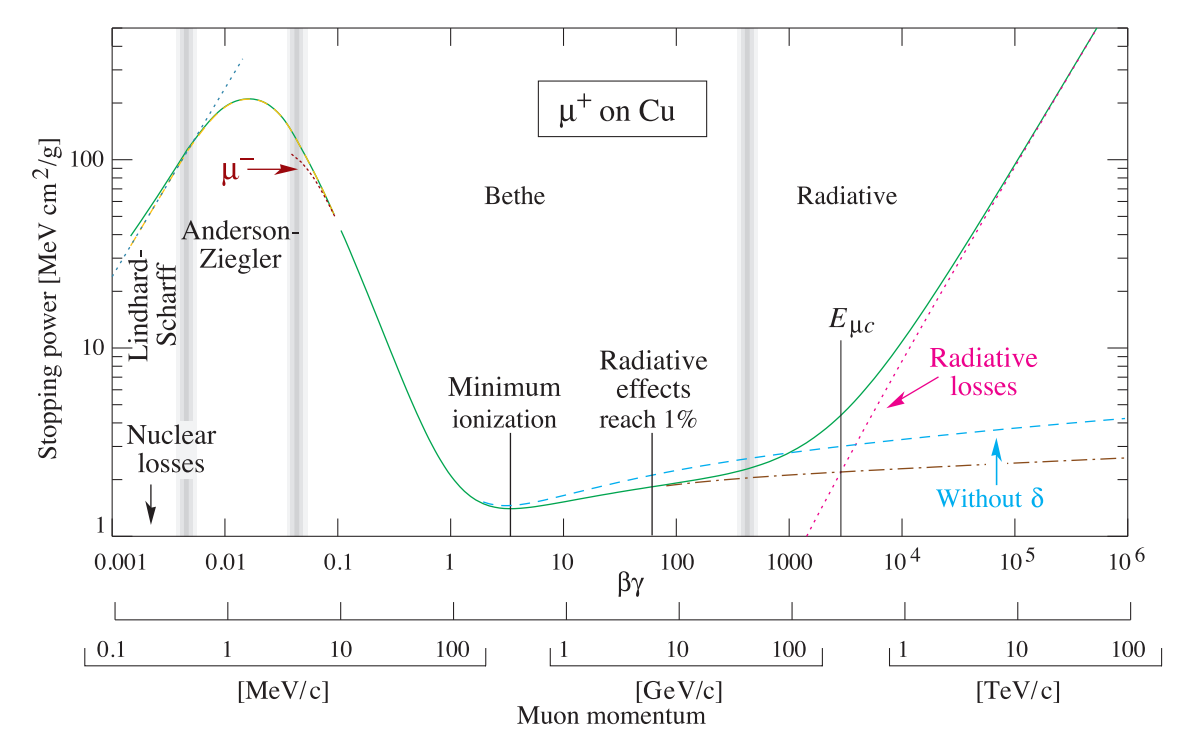
\includegraphics[width=.9\textwidth]{images/mu-pi-bethe.png}
  \caption{Energy loss by a muon in copper as a function of \( \beta\gamma \) or momentum. The solid line indicates the total stopping power, dashed lines indicate different contributions and the vertical grey bands indicate the different phenomenological regimes. Taken from ref~\cite{PDG particles in matter ref}.}
  \label{fig:mu-pi-bethe}
\end{figure}
\begin{figure}[hptb]
  \centering  
    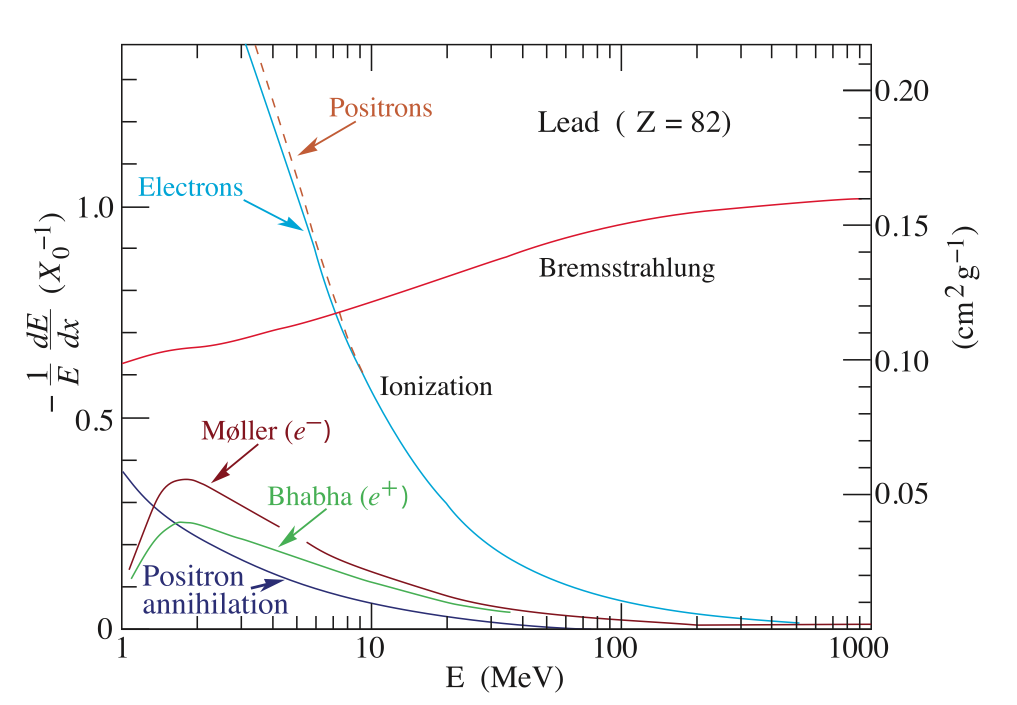
\includegraphics[width=.9\textwidth]{images/electron_energy_loss.png}
  \caption{Electron energy loss per `radiation length' (\( X_0^{-1} \)) as a function of electron energy (not momentum). The material in this case is lead (\(Z=82\) and \(X_0 = 6.37\)g/cm\(^2\)). Taken from ref~\cite{PDG particles in matter ref}.}
  \label{fig:electron_energy_loss}
\end{figure}

At MuSIC the loss of energy by charged particles to matter is very important as it is the main method for detecting, and hence, characterising, the beam. The main method of detection used at MuSIC is via scintillation light: when a particle deposits energy in a certain materials (bit it via ionisation or some other method) they will produce light, this light can then be detected giving information on the beam. The largest problem for this technique is the plateau seen in the distributions for muons and pions: when these particles are minimally ionising they can be difficult to detect so this has to be accounted for. 
 
% section charged_particle_interactions_in_matter (end)
%%%%%%%%%%%%%%%%%%%%%%%%%%%%%%%%%%%%%%%%%%%%%%%%%
\section{Muon decay} % (fold)
\label{sec:muon_decay}
As has been noted muons decay 99\% of the time through the process: \( \mu \rightarrow \nu \nu e \). This process is the same for both positive and negative muons although there is a sign change and the flavour of the anti-neutrino will swap. The biggest difference between positive and negative muons is that negative muons can become bound to a nucleus in a an analogous situation to electrons. This section will start with a general discussion of the important parameters of muon decay and then continue with a discussion of how this property of negative muons changes their decay.

The decay of a muon, like any other decay, can be modelled using a poisson distribution:
\begin{equation}\label{eq:poisson}
  P(t) = Ne^{-t/\tau}
\end{equation}
Where \( P(t) \) is the survival probability of a particle after time, \( t \); \( N \) is a scaling factor to the size of the initial population and \( \tau \) is the population's lifetime. For a free muon in a vacuum the lifetime is \( \sim2.2\)~\( \mu \)s. As figure~\ref{fig:muon_decay_feynmann} shows the muon decay is mediated by a charged W boson, the presence of the two neutrinos mean that the only practically detectable result of the muon decay is the electron. The muons (comparatively) long lifetime makes identification of them possible through by plotting decay times, this is discussed in greater detail in part~\ref{prt:characterising_the_beam}. 

\begin{figure}[hptb]
  \centering
    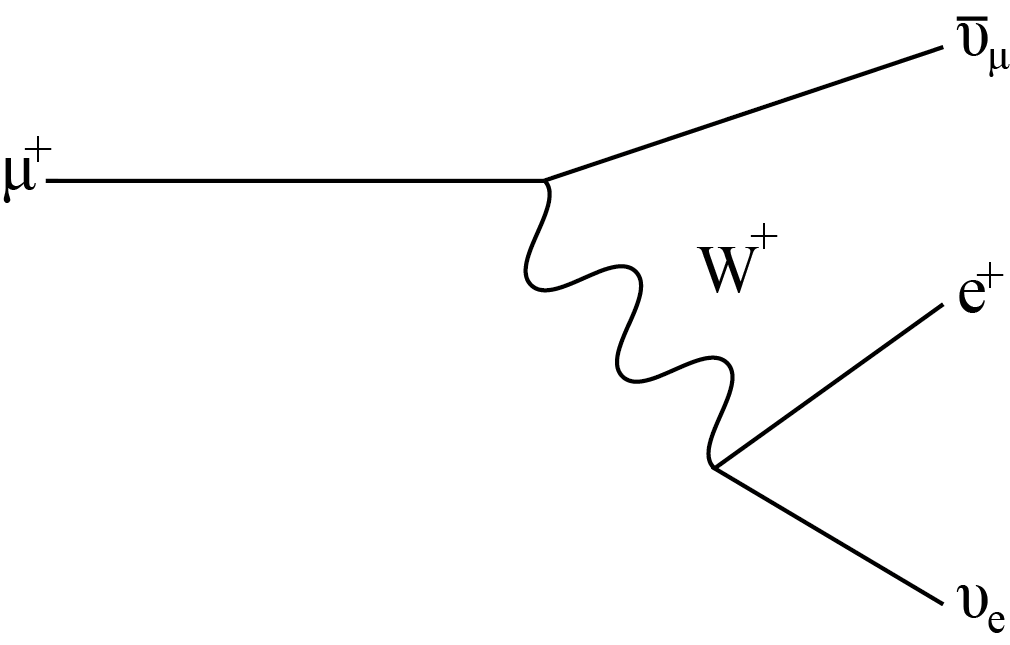
\includegraphics[scale=1]{images/muon_decay_feynmann.png}
  \caption{Feynman diagram showing muon decay.}
  \label{fig:muon_decay_feynmann}
\end{figure}

As has been noted negative muons can undergo an additional interaction with matter compared to positive muons. As a negatively charged lepton they can be become bound to a nucleus, reducing its lifetime. The muon lifetime can be expressed as the reciprocal of an interaction rate:
\begin{equation}\label{eq:capture_rate}
  \tau_{\mu^-} = (\Delta_t)^{-1}
  \Delta_t = \Delta_c + Q\Delta_d
\end{equation}
where \( \Delta_t \) is the total interaction rate; \( \Delta_c \) is the rate of nuclear muon capture; \( Q\Delta_d \) is the rate of decay for positive muons (i.e.\ \( \tau_{\mu^+} = (\Delta_d)^{-1}  \)) modified by the `Huff-factor', \( Q \), which compensates for the reduction in energy available for a bound muon to decay. 

A theoretical approximation to \( \Delta_c \) as a function of atomic mass, \( A \), and atomic number, \( Z \), was devised by Primakoff and Goulard~\cite{primakoff_and_goulard}:
\begin{equation}\label{eq:primakoff_and_goulard}
  \Delta_c(A,Z)=Z^4_{eff} G_1 \left[ 1 + G_2 \frac{A}{2Z} - G_3 \frac{A-2Z}{2Z} - G_4 \left[\frac{A-Z}{2A} + \frac{A-2Z}{8AZ} \right] \right]
\end{equation}
Where \( Z_{eff} \) is the effective value for the atomic number as calculated by Ford and Wells~\cite{Wells and ford Zeff} that accounts for the muon's orbital radius being comparable to the nucleus'. The difference between the predicted capture rate and the measured rate is given in figure~\ref{fig:primakoff-goulard_vs_exp} with the fitted values show in table~\ref{tab:g1_to_g4}. When a negative muon is captured by a nucleus its lifetime is reduced compared to the positive muon. This reduction is due to the muon forming a muonic atom with its captor that allows it to rapidly shed energy via X-rays as it cascades through various shells until it enters the \( 1s \) state. The muonic cascade is a very rapid event, in most materials it occurs in less than \( 10^{-13}\)s~\cite{nuclear physics of muon capture}, once in the \( 1s \) state the muon will decay much sooner having lost most of its energy.

\begin{figure}[hptb]
  \centering
    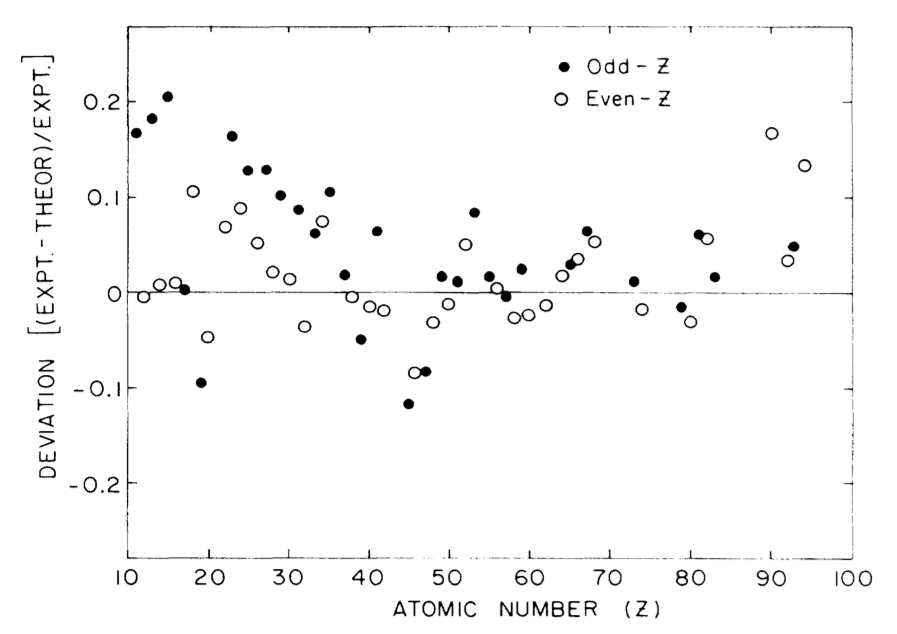
\includegraphics[width=.9\textwidth]{images/primakoff-goulard_vs_exp.png}
  \caption{Comparison of the theoretical values (as determined using the Primakoff-Goulard formula) and experimentally determined capture rates for a range of materials, taken from~\cite{Suzuki total nuclear capture rate}.}
  \label{fig:primakoff-goulard_vs_exp}
\end{figure}

\begin{table}
  \begin{center}
  \begin{tabular}{c | r@{.}l | r@{.}l }
                                                              & \multicolumn{2}{c|}{TRIUMF data} & \multicolumn{2}{c}{Past Results}  \\
    \hline
    Number of data                                            & \multicolumn{2}{c|}{30}          & \multicolumn{2}{c}{58}            \\
    \hline
    \( G_1 \)                                                 &             260 &                &              252 &                \\
    \( G_2 \)                                                 &              -0 & 040            &               -0 & 038            \\
    \( G_3 \)                                                 &              -0 & 26             &               -0 & 24             \\
    \( G_4 \)                                                 &               3 & 24             &                3 & 23             \\
    \hline
    \( (\textrm{Expt.} - \textrm{Fit})/\textrm{Expt.} \) (\%) &               4 & 1              &                5 & 6              \\
  \end{tabular}
  \end{center}
  \caption{Experimentally determined values of \( G_1 \)--\( G_4 \) as determined by TRIUMF~\cite{Suzuki total nuclear capture rate}.}
  \label{tab:g1_to_g4}
\end{table}


% section muon_decay (end)
%%%%%%%%%%%%%%%%%%%%%%%%%%%%%%%%%%%%%%%%%%%%%%%%%%%
% chapter physics (end)
%%%%%%%%%%%%%%%%%%%%%%%%%%%%%%%%%%%%%%%%%%%%%%%%%%%
% part introduction (end)
%%%%%%%%%%%%%%%%%%%%%%%%%%%%%%%%%%%%%%%%%%%%%%%%%%%